\section{Differential Datalog (DDlog)}\label{sec-ddlog}

A DDlog program operates on typed relations.  The programmer defines a
set of rules to compute a set of output relations based on input
relations (Figure~\ref{fig:differential}).  Rules are evaluated
incrementally: given a set of \emph{changes} to the input relations
(insertions or deletions), DDlog produces a set of changes to the
output relations (expressed also as insertions or deletions).

\begin{figure}[t]
    \center
    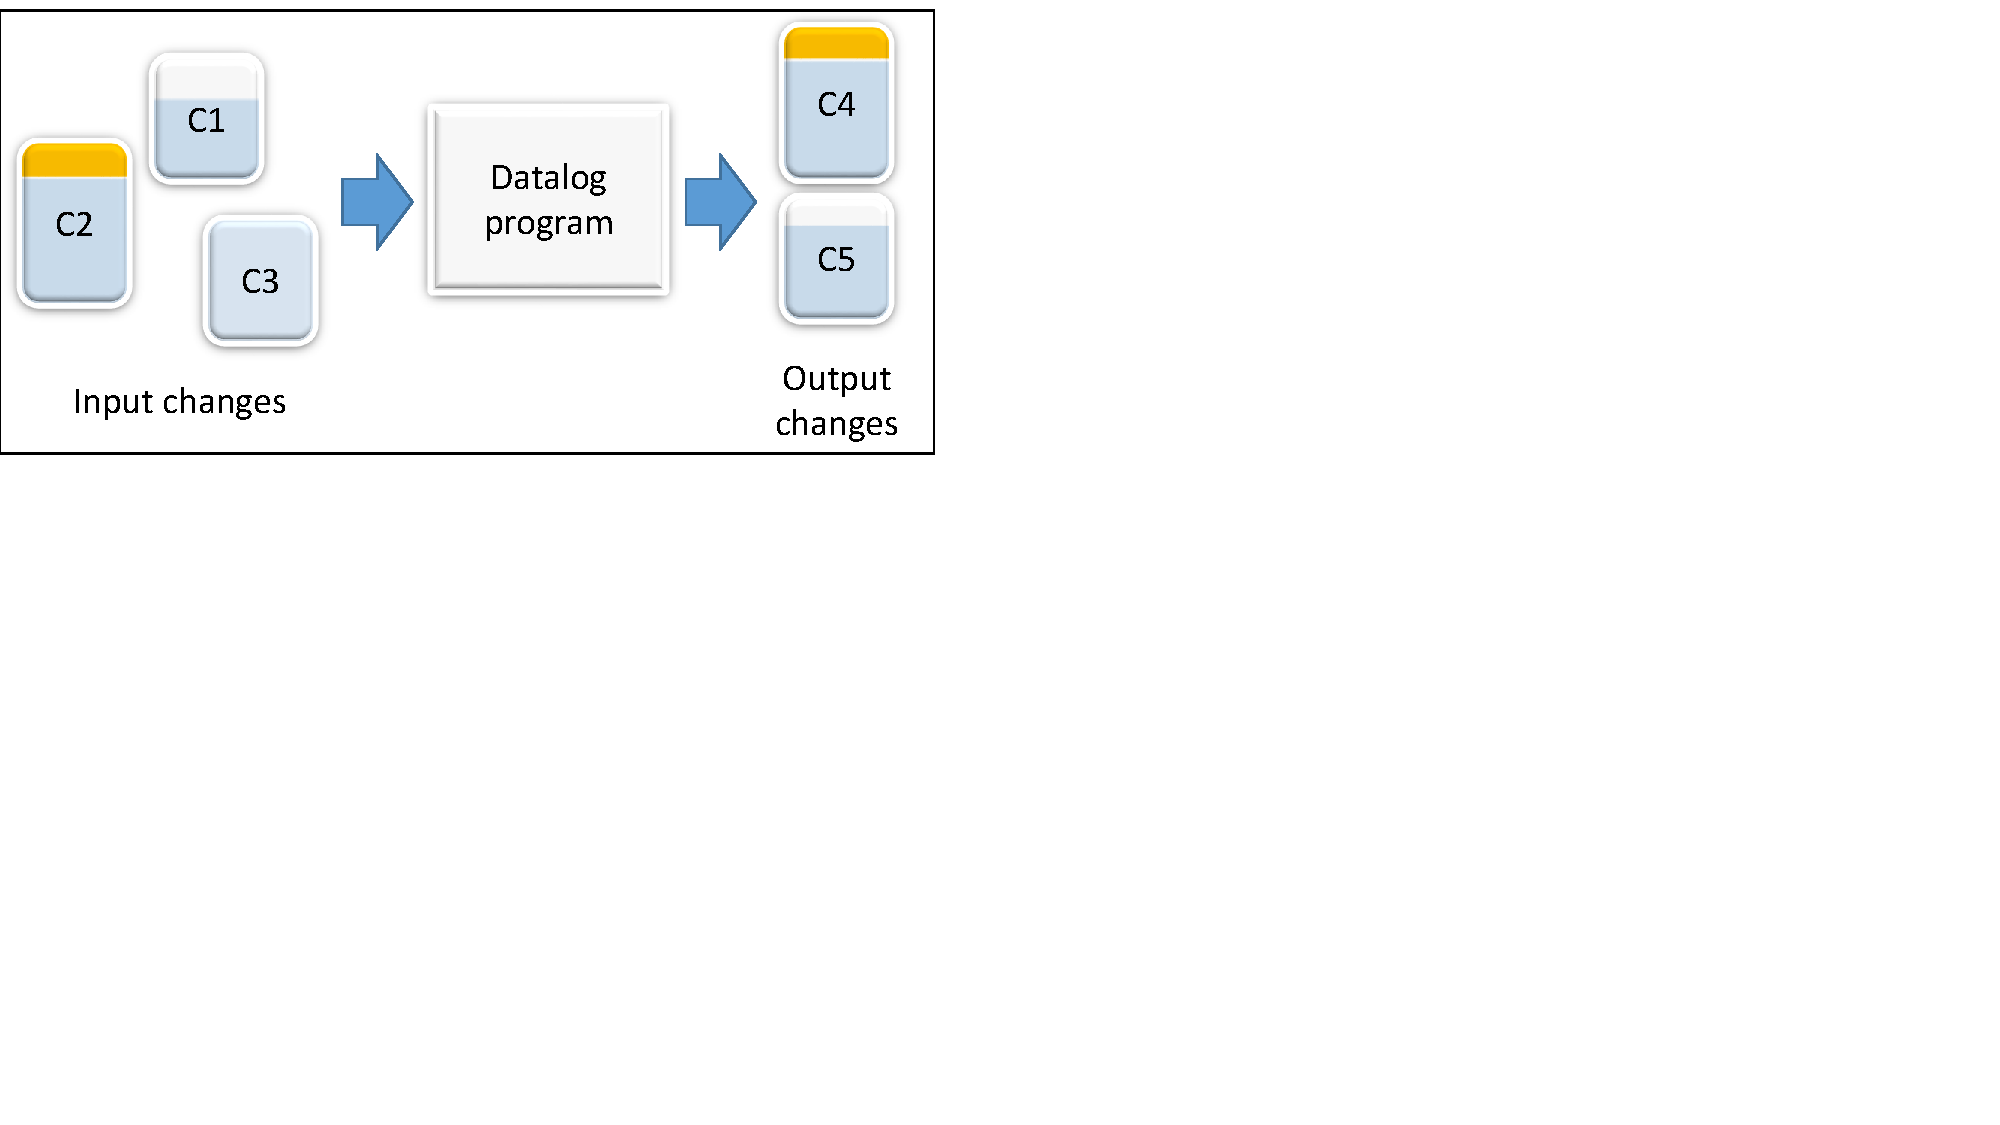
\includegraphics[width=0.5\columnwidth,clip=true,trim=0in 4.4in 6.5in 0in]{differential.pdf}
    \caption{Incremental evaluation of a Datalog program.\label{fig:differential}}
\end{figure}

In this section we give a brief overview of the language; we refer the
reader to the DDlog language reference~\cite{ddlog-manual} and the DDlog
tutorial~\cite{ddlog-tutorial} for a detailed presentation of language
features.

%\subsection{Syntax}
%
%DDlog is case-sensitive.  Relation, constructor, and type variable
%names must start with upper-case ASCII letters; variable, function,
%and argument names must start with lower-case ASCII letters or
%underscore.  A type variable name must be prefixed with a tick
%(\texttt{'}). A type name can start with either an upper-case or a
%lower-case letter or underscore.  Names must be unique within a scope.

\subsection{Type system}

DDlog is a strongly-typed language.  DDlog performs type inference,
but users can specify the types of expressions explicitly as well.
All programs are type-checked statically.  The type system is inspired
by Haskell, and supports a rich set of types.  Base types include
Booleans, bit-strings, e.g., \texttt{bit<32>}, infinite-precision
integers \texttt{bigint}, UTF-8 strings.  Derived types are tuples,
structures, and tagged unions (which generalize enumerated types).  We
do not allow defining recursive types like lists or trees; however
it provides three built-in collection types: maps, sets, and arrays
(Section~\ref{sec:collections}).

Figure~\ref{fig:types} shows several type declarations.  DDlog
supports also generic types; type variables are preceded by a tick:
\texttt{'A}.  The language contains a built-in reference type
\texttt{Ref<'T>}.  Unlike other languages, two references are equal if
the objects referred are equal; thus references do not alter the
nature of Datalog in any significant way.  References can be used to
reduce memory consumption when complex objects are stored in multiple
relations.

\begin{figure}[t]
  \small
\begin{lstlisting}[language=ddlog]
// A tagged-union type
typedef IPAddress = IPv4Address{ipv4addr: bit<32>}
                  | IPv6Address{ipv6addr: bit<128>}
// A generic option type
typedef Option<'A> = None
                   | Some{value: 'A}
typedef OptionalIPAddress = Option<IPAddress>                   
\end{lstlisting}
\caption{Some type declarations in DDlog.\label{fig:types}}
\end{figure}

\subsection{Relations}

Relations are strongly typed; the value in each column must have a
statically-determined type.  There are three kinds of relations in
DDlog:
\begin{description}
\item[Input relations:] the contents of these relations is provided by
  the environment of the program.
\item[Output relations:] these must be computed by the DDlog program, and the
  DDlog runtime will inform the environment of any changes that
  occur in these relations.
\item[Intermediate results:] these must be also computed by the DDlog
  program, but the environment cannot query the contents of these
  relations.
\end{description}

Figure~\ref{fig:relations} shows example relation declarations.  An
input relation may declare an optional primary key --- which is a set
of columns that can be used to delete entries more efficiently,
specifying only the key.

\begin{figure}[t]
  \small
  \begin{lstlisting}[language=ddlog]
input relation Edge(from: node_t, to: node_t)
               primary key (e) e.from
output relation Path(src: node_t, dst: node_t)
  \end{lstlisting}
  \caption{Example relation declarations.\label{fig:relations}}
\end{figure}

\subsection{Rules}

DDlog rules are composed of standard Datalog operators: joins, antijoins, and
unions, illustrated in Figure~\ref{fig:rules}, as
well as aggregation, and flatmap, discussed in Section~\ref{sec:collections}.
DDlog allows recursive rules with stratified negation: intuitively, a DDlog
relation cannot recursively depend on its own negation.

\begin{figure}[t]
  \small
  \begin{lstlisting}[language=ddlog]
/* The Path relation is computed as a union of two rules */

// Rule 1: base case
Path(x, y) :- Edge(x,y).

// Rule 2: recursive step: join Path relation with Edge
// followed by an antijoin with Exclude to ignore nodes
// in the Exclude relation.
Path(x, z) :- Path(x, w), Edge(w, z), not Exclude(z).
  \end{lstlisting}
  \caption{Example DDlog rules that compute the set of paths in a graph.\label{fig:rules}}
\end{figure}

\subsection{Expressions}

Much of DDlog's power stems from its ability to perform complex computation
inside rules.  For example, the rule in Figure~\ref{fig:area} computes
an inner join of height and width tables using the object id column and
then computes the area of the object as the product of its height and width.
This is in contrast to the textbook Datalog that is limited to selecting
columns from existing relations.

\begin{figure}[t]
  \small
  \begin{lstlisting}[language=ddlog]
input relation Height(object_id: int, height: int)
input relation Width(object_id: int, width: int)
output relation Area(object_id: int, area: int)

// Compute the area of an object as the product of
// its height and width.
Area(oid, area) :- Height(oid, h), Width(oid, w),
                   var area = w * h.
  \end{lstlisting}
  \caption{Using expressions in a rule.\label{fig:area}}
\end{figure}

The full DDlog expression language supports arithmetics, string manipulation, control
flow constructs and function calls.

%DDlog is an expression-oriented language; programs are composed of
%expressions, that evaluate to ground values.  Sequential composition
%of two expressions (written using semicolon) evaluates to the last
%expression.

\paragraph{Arithmetics}
The arithmetic types (\texttt{bigint} and \texttt{bit<N>}) provide the
standard arithmetic operations, as well as bit-wise operations, bit selection
\texttt{v[15:8]}, shifting, and concatenation.

\paragraph{Strings} All primitive types contain built-in conversions to strings, and users
can implement string conversion functions for user-defined types
(like Java's toString() method).

Expressions enclosed within \texttt{\$\{...\}} in a string literal are
\emph{interpolated}: they are evaluated at run-time, converted to
strings and substituted; this is a feature inspired by JavaScript; for
example \texttt{"x+y=\$\{x+y\}"}.

\paragraph{Control flow}

DDlog is an expression-oriented language, meaning that any expression
evaluates to a ground value and can be used, e.g., in the righ-hand side
of an assignment.  Similar to other expression-oriented languages,
DDlog supports \texttt{if-else} expressions, where the \texttt{else} branch
must be present.

Inspired by ML and Haskell, the DDlog \texttt{match} expression
simultaneously performs pattern-matching against type constructors or
values and value binding.  Figure~\ref{fig:function} shows a
\texttt{match} expression that uses a nested pattern to extract a byte from
\texttt{OptionalIPAddress}.  This pattern binds the \texttt{addr}
variable.

\begin{figure}[t]
  \small
  \begin{lstlisting}[language=ddlog]
function lastByte(a: OptionalIPAddress): bit<8> = {
  match (a) {
    None -> 0,
    Some{IPv4Address{.ipv4addr = addr}} -> addr[7:0],
    Some{IPv6Address{.ipv6addr = addr}} -> addr[7:0]
  }
}
  \end{lstlisting}
\caption{A DDlog function using pattern matching.\label{fig:function}}
\end{figure}

Pattern matching can also be used directly in the body of a rule.  For example,
the following rule extracts only IPv6 addresses from the \texttt{Host}
relation.

\begin{lstlisting}[language=ddlog]
IPv6Addr(addr):-Host(.address=Some{IPv6Address{addr}}).
\end{lstlisting}

Finally, programmers can use \texttt{for} loops to iterate
over elements of collections, as explained in Section~\ref{sec:collections}
below.

\paragraph{Local variables}

Local variables are used to store intermediate results of computations.
In DDlog, local variables can be introduced in three different contexts.  First,
variables can be defined directly in the body of a rule, e.g., the \texttt{area}
variable in Figure~\ref{fig:area}.  Second, they can be defined inside
an expression, e.g., the \texttt{res} variable in Figure~\ref{fig:collections}.
Third, a variable can be defined in a \texttt{match} pattern,
as in Figure~\ref{fig:function}.
A local variable is visible within the syntactic scope where it was defined.

\subsection{Functions}

DDlog functions encapsulate pure (side-effect-free) computations.  
An example function is shown in
Figure~\ref{fig:function}.  Recursive functions are not supported.
Users and libraries can declare prototypes of \texttt{extern}
functions, which must be implemented outside of DDlog (e.g., in Rust),
and linked against the DDlog program at link time.  The compiler
assumes that extern functions are pure.

\subsection{Collections}\label{sec:collections}

The DDlog standard library contains three built-in generic collection
types (implemented natively in Rust): \texttt{Vec<'T>},
\texttt{Set<'T>} and \texttt{Map<'T>}.  Values of these types can be
stored as first-class values within relations.  Equality for values
of these types is defined as expected, element-wise.  In theory such
types are not necessary, since collections within relations can be
represented using separate relations.  We have
introduced them into the language because many practical applications
have data models that contain nested collections; by supporting
collection-valued columns natively in DDlog we can more easily
interface with such applications, without the need to write glue code
to convert collections back and forth into separate relations using
foreign keys.

%The downside of using collections as relation values is
%that DDlog does not compute incremental changes of collections (only
%incremental changes to relations).

Figure~\ref{fig:collections} shows the declaration in DDlog of an
external function which splits a string into substrings using a
separator; this function returns a vector of strings.

\begin{figure}[t]
  \small
  \begin{lstlisting}[language=ddlog]
// declare external function returning a vector of strings
extern function split(s: string, sep: string): Vec<string>
// DDlog function to concatenate all elements of a vector
function concat(s: Vec<string>, sep: string): string = {
  var res = "";
  for (e in s) {
    res = if (res != "") res + sep else res;
    res = res + e
  };
  res   // last value is function evaluation result
}

input relation Phrases(p: string)
relation Words(w: string)
// Words contains all words that appear in some phrase
Words(w) :- Phrases(p), var w = FlatMap(split(p, " ")).

// Shortest path between each pair of points x, y
// (x, y) is the key for grouping
// min is the function used to aggregate data in each group
ShortestPath(x, y, min_cost) :- Path(x, y, cost),
                 var min_cost = Aggregate((x, y), min(cost)).
\end{lstlisting}
\caption{Operations on collections: iteration, flattening,
  aggregation.\label{fig:collections}}
\end{figure}

\texttt{for} loops can be used to iterate over elements in
collections.  Figure~\ref{fig:collections} shows an implementation of
the function \texttt{concat}, the inverse of \texttt{split} using a
loop.

The \texttt{FlatMap} operator can be used to flatten
a collection into a set of DDlog records, as illustrated in the definition of
relation \texttt{Words} in Figure~\ref{fig:collections}.

The \texttt{Aggregate} operator can be used to evaluate the equivalent
of SQL groupby-aggregate queries.  The aggregate operator has two
arguments: a key function, and an aggregation function.  The
aggregation function receives a group of
records that share the same key.  The
\texttt{ShortestPath} relation in Figure~\ref{fig:collections} is
computed using aggregation.

\subsection{Module system}

DDlog offers a simple module system, inspired by Haskell and Python,
which allows importing definitions (types, functions, relations) from
multiple files.  The user can add imported definitions directly into the
name space of the importing module or keep them in a separate name space to
prevent name clashes.  Similar to Java packages, module names are
hierarchical and the module name hierarchy must match the paths on the
the filesystem where modules are stored.  The directive \texttt{import
  library.module} will load the module from file
\texttt{library/module.dl}.  The standard library itself is a module
named \texttt{std}.

\subsection{``Imperative'' relation definitions}

We have also defined an alternative syntax for rules,
inspired by the FLWOR syntax of XQuery expressions; an example is
given in Figure~\ref{fig:imperative}.  This is just syntactic sugar,
entirely eliminated by the compiler front-end.  The ``imperative''
fragment offers several statements: \texttt{skip} (does nothing),
\texttt{for}, \texttt{if}, \texttt{match}, block statements (enclosed
in braces), and variable definitions \texttt{var...in}.  Note that
these are \emph{statements}, and are syntactically different from the
similar \emph{expressions} \texttt{for}, \texttt{var}, \texttt{match},
\texttt{if}.

\begin{figure}[t]
  \small
  \begin{lstlisting}[language=ddlog]
for (region in Region) 
    for (person in Person(.region = region.id))
        var is_audience = is_targeted(person) in
        match (is_audience) {
           true -> TargetAudience(person)
           _    -> skip
        }    
  \end{lstlisting}
  \caption{Imperative-style code defining relation TargetAudience.\label{fig:imperative}}
\end{figure}

\subsection{The standard library}

The DDlog standard library has a growing collection of useful
functions and data structures: some generic functions and data-types,
such as \texttt{min}, string manipulation and conversion to strings,
functions to manipulate vectors, sets, maps (insertion, deletion,
lookup, etc.).
